\documentclass[a4paper,11pt]{article}
\usepackage{amsmath,amsthm,amsfonts,amssymb,amscd,amstext,vmargin,graphics,graphicx,tabularx,multicol} 
\usepackage[francais]{babel}
\usepackage[utf8]{inputenc}  
\usepackage[T1]{fontenc} 
\usepackage{pstricks-add,tikz,tkz-tab,variations}
\usepackage[autolanguage,np]{numprint} 
\usepackage{calc}

\setmarginsrb{1.5cm}{0.5cm}{1cm}{0.5cm}{0cm}{0cm}{0cm}{0cm} %Gauche, haut, droite, haut
\newcounter{numexo}
\newcommand{\exo}[1]{\stepcounter{numexo}\noindent{\bf Exercice~\thenumexo} : }
\reversemarginpar

\newcommand{\bmul}[1]{\begin{multicols}{#1}}
\newcommand{\emul}{\end{multicols}}

\newcounter{enumtabi}
\newcounter{enumtaba}
\newcommand{\q}{\stepcounter{enumtabi} \theenumtabi.  }
\newcommand{\qa}{\stepcounter{enumtaba} (\alph{enumtaba}) }
\newcommand{\initq}{\setcounter{enumtabi}{0}}
\newcommand{\initqa}{\setcounter{enumtaba}{0}}

\newcommand{\be}{\begin{enumerate}}
\newcommand{\ee}{\end{enumerate}}
\newcommand{\bi}{\begin{itemize}}
\newcommand{\ei}{\end{itemize}}
\newcommand{\bp}{\begin{pspicture*}}
\newcommand{\ep}{\end{pspicture*}}
\newcommand{\bt}{\begin{tabular}}
\newcommand{\et}{\end{tabular}}
\renewcommand{\tabularxcolumn}[1]{>{\centering}m{#1}} %(colonne m{} centrée, au lieu de p par défault) 
\newcommand{\tnl}{\tabularnewline}

\newcommand{\trait}{\noindent \rule{\linewidth}{0.2mm}}
\newcommand{\hs}[1]{\hspace{#1}}
\newcommand{\vs}[1]{\vspace{#1}}

\newcommand{\N}{\mathbb{N}}
\newcommand{\Z}{\mathbb{Z}}
\newcommand{\R}{\mathbb{R}}
\newcommand{\C}{\mathbb{C}}
\newcommand{\Dcal}{\mathcal{D}}
\newcommand{\Ccal}{\mathcal{C}}
\newcommand{\mc}{\mathcal}

\newcommand{\vect}[1]{\overrightarrow{#1}}
\newcommand{\ds}{\displaystyle}
\newcommand{\eq}{\quad \Leftrightarrow \quad}
\newcommand{\vecti}{\vec{\imath}}
\newcommand{\vectj}{\vec{\jmath}}
\newcommand{\Oij}{(O;\vec{\imath}, \vec{\jmath})}
\newcommand{\OIJ}{(O;I,J)}


\newcommand{\reponse}[1][1]{%
\multido{}{#1}{\makebox[\linewidth]{\rule[0pt]{0pt}{20pt}\dotfill}
}}

\newcommand{\titre}[5] 
% #1: titre #2: haut gauche #3: bas gauche #4: haut droite #5: bas droite
{
\noindent #2 \hfill #4 \\
#3 \hfill #5

\vspace{-1.6cm}

\begin{center}\rule{6cm}{0.5mm}\end{center}
\vspace{0.2cm}
\begin{center}{\large{\textbf{#1}}}\end{center}
\begin{center}\rule{6cm}{0.5mm}\end{center}
}



\begin{document}
\pagestyle{empty}
\titre{Séance d'AP 2  : Statistiques et tableur}{}{}{3ème}{}

\vspace*{0.2cm}

\textbf{{\large Partie A}}\\

On considère une entreprise dont le tableau ci-dessous donne la répartition des salaires mensuels pour l'année 2004 en fonction de la catégorie des employés.\\

\q Recopier le tableau suivant dans le tableur. 

\begin{flushleft}
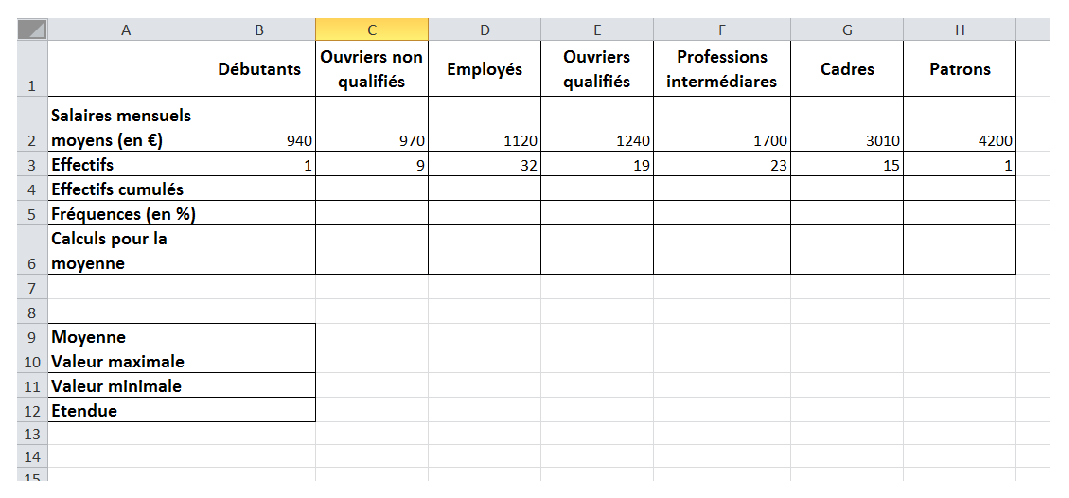
\includegraphics[scale=1]{stat1.eps} 
\end{flushleft}

\textit{Astuce pour aller automatiquement à la ligne dans une cellule : Sélectionne les cellules où tu souhaites un renvoi à la ligne puis va dans Format – Alignement. Dans l'onglet alignement, coche la case "renvoi à la ligne dans la cellule".}\\


\q On se propose de compléter automatiquement la ligne  \textbf{"effectifs cumulés"}.\\

\qa  Pour compléter la cellule \textbf{B4}, écrire la formule suivante : \textbf{=B3}.\\

\qa Dans chacune des cellules \textbf{C4} à \textbf{H4} on veut obtenir la somme du nombre contenu dans la cellule de gauche et du nombre contenu dans la cellule au-dessus. Pour obtenir ce résultat :
\bi
\item Placer dans la cellule \textbf{B4} la formule \textbf{= B3} (après avoir tapé une formule, taper toujours sur la touche Entrée).
\item Placer dans la cellule \textbf{C4} la formule \textbf{=C3+B4}
\item Sélectionner ensuite la cellule \textbf{C4} et étendre cette formule jusqu'à la cellule \textbf{H4} (\textbf{voir information ci-dessous}). Vérifier alors que la cellule \textbf{H4} contient la formule \textbf{=H3+G4}. 
\ei


\setlength{\fboxrule}{2pt}
\begin{flushleft}
\framebox{\begin{minipage}{\linewidth}

\vspace*{0.2cm}
\textbf{Info :} cette opération s'effectue avec la souris en sélectionnant la cellule \textbf{C4} et en tirant "le petit carré noir" dans l'angle inférieur droitde la cellule jusqu'à la cellule \textbf{H4}.


\vspace*{0.2cm}
\end{minipage}}
\end{flushleft}

\vspace*{0.2cm}

\q  Dans quelle cellule peut-on lire l'effectif total de la série ? . . . . . . . . . . . . . .\\
Combien vaut-il ? . . . . . . . . . . . . . . . . . . . . . . . . . . . . . . \\

\q  On se propose de compléter automatiquement la ligne  \textbf{"Fréquences"}.\\
 Quelle formule doit-on écrire dans la cellule \textbf{B5} ? . . . . . . . . . . . . . . . . . . . . . . . . \\
 Avec la même technique que ci-dessus, compléter la ligne des fréquences automatiquement.\\
 
 \newpage

 
  \setlength{\fboxrule}{2pt}
\begin{flushleft}
\framebox{\begin{minipage}{\linewidth}

\vspace*{0.2cm}
\textbf{Définition :} La médiane d'une série statistique est le nombre qui partage cette série en deux groupes de même effectif.

\vspace*{0.2cm}
\end{minipage}}
\end{flushleft}
 \q  \initqa \qa  Quand on utilise les effectifs cumulés, comment peut-on déterminer la médiane ? . . . . . . . . . . . . . . . . . . . . . . . . . . . . . . . . . . . . . . . . . . . . . . . . . . . . . . . . . . . . . . . . . . . . . . . . . . . . . . . . . . . . . . . . . . . . . . . . . . . . . . . . . . . . . . . . . . \\
 
\qa Quel est le salaire médian de cette entreprise ? . . . . . . . . . . . . . . . . \\

\q  \initqa \qa Pour obtenir la moyenne, on va entrer des calculs intermédiaires dans \textbf{la ligne 6}.\\
- Ainsi dans la cellule \textbf{B6}, on entre \textbf{=B2*B3}.
Quelle formule doit-on entrer dans la cellule \textbf{C6} ? . . . . . . . . . . .\\
- Étendre la formule jusqu'à la cellule \textbf{H6}.\\
- Pour obtenir la somme des valeurs de la ligne 6, entrer dans la cellule \textbf{I6} la formule \textbf{=SOMME(B5:H5)}.\\

\qa Quelle formule doit-on entrer dans la cellule \textbf{B9} pour obtenir la moyenne ? . . . . . . . . . . . . . . . . . .\\

\qa Entrer la formule trouvée dans la cellule \textbf{B9}. Quelle est la moyenne obtenue ? . . . . . . . . . . . . . . . . . \\ 

\q  On observe alors un écart assez important entre le salaire médian et le salaire moyen. Comment peut-on l'expliquer ?\\
\reponse[2]\\

\q  \initqa \qa Dans la cellule \textbf{B10}, entrer la formule \textbf{ =MAX(B2:H2)}.\\
 Quelle valeur obtient-on et que représente-t-elle ? . . . . . . . . . . . . . . . . . . . . . . . . . . . . . \\
 
\qa Dans la cellule \textbf{B11}, entrer la formule \textbf{=MIN(B2:H2)}.\\
 Quelle valeur obtient-on et que représente-t-elle ? . . . . . . . . . . . . . . . . . . . . . . . . . . . . . 
 
 
 \setlength{\fboxrule}{2pt}
\begin{flushleft}
\framebox{\begin{minipage}{\linewidth}

\vspace*{0.2cm}
\textbf{Définition :} L'étendue d'une série statistique est la différence entre sa valeur la plus élevée et sa valeur la plus basse. 


\vspace*{0.2cm}
\end{minipage}}
\end{flushleft}
 
 \q \initqa \qa Quelle formule doit-on entrer en \textbf{B12} pour obtenir l'étendue de la série ? . . . . . . . . . . . . . . . . \\
 
\qa Quelle est l'étendue de cette série ?  . . . . . . . . . . . . . . . . .\\


\textbf{{\large Partie B}}\\

Nous allons maintenant voir l'utilité de rentrer ces formules dans le tableur. En 2005, le patron de l'entreprise a décidé de modifier les salaires et le nombre de salariés a changé. Voici les nouvelles données. \\

\begin{flushleft}
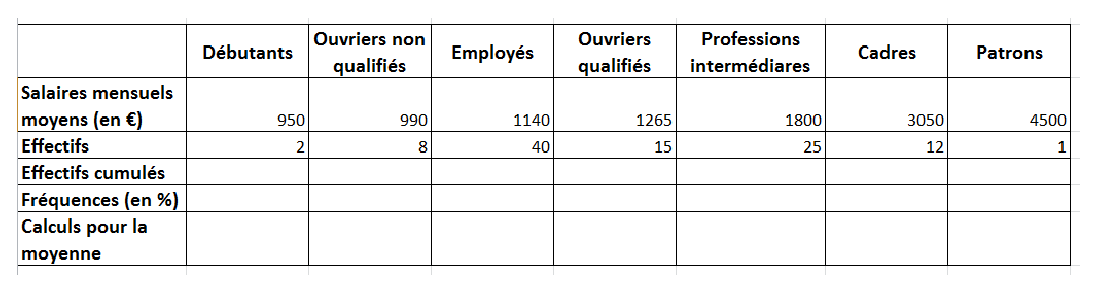
\includegraphics[scale=1]{stat2.eps} 
\end{flushleft}

\initq \q \initqa \qa Modifier les lignes 2 et 3 du tableau à l'aide des nouvelles données. Grâce aux formules que vous avez entrées, les effectifs cumulés, la moyenne et l'étendue sont recalculées automatiquement.\\

\newpage

\vspace*{0.4cm}

\qa Compléter maintenant le tableau ci-dessus avec les nouvelles valeurs trouvées.\\
- Quelle est la nouvelle moyenne obtenue ? . . . . . . . . . . . . . . . . .\\
- Quelle est la nouvelle étendue ? . . . . . . . . . . . . . . . .\\
- Par simple lecture de ce tableau, donner le nombre de personnes ayant un salaire inférieur à 1800 euros :  . . . .\\


\q  Pour finir, nous aller créer un diagramme en bâtons représentant les effectifs des salaires moyens de l'entreprise en 2005.\\

- Pour cela, sélectionner la ligne 3 de la feuille de calcul, aller dans \textbf{Insertion} et cliquer sur \textbf{Histogramme}.  \\
Cliquer droit sur l'histogramme puis cliquer sur \textbf{Sélectionner des données}. Nous allons pour finir modifier l'axe horizontal en sélectionnant la ligne 2 des salaires mensuels.\\ 


- Enregistrer votre travail. \\

\vspace*{0.5cm}

\begin{center}
\textbf{\underline{{\large Pour ceux qui vont plus vite}}}
\end{center}

\vspace*{0.3cm}

Le tableau ci-dessous fournit, pour la France, la vitesse moyenne des
véhicules légers, ainsi que le nombre de morts sur les routes, de 1998 à 2006.\\

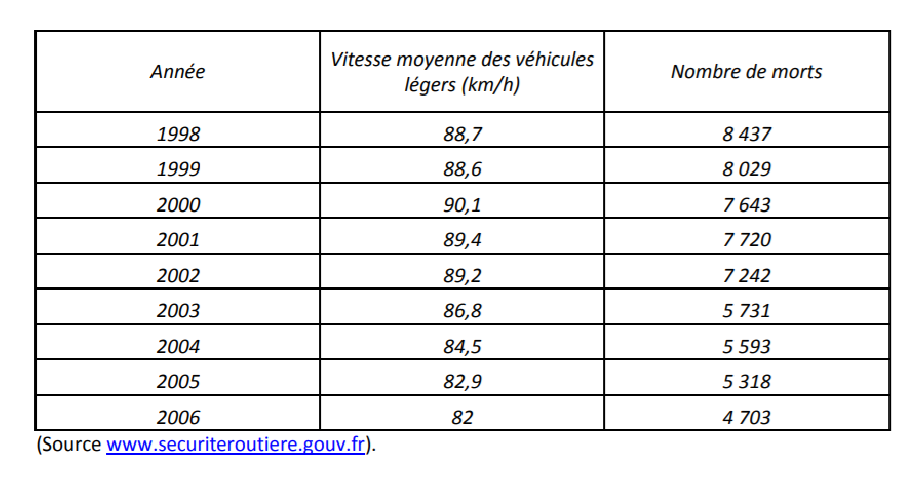
\includegraphics[scale=0.9]{stat3.eps} \hspace*{0.5cm} 
\includegraphics[scale=0.75]{stat4.eps}\\

\initq \q \initqa \qa Représenter, à l'aide d'un tableur, l'évolution de la vitesse moyenne en fonction des années (choisir un « nuage de points reliés par
une courbe »).\\

\qa Représenter de même l'évolution du nombre de morts en fonction des années.\\

\qa Comparer les deux graphiques.\\
\reponse[3]\\

\q \initqa \qa Représenter, à l'aide d'un tableur, le nuage de points (non reliés) correspondant à la série statistique à deux variables, vitesse et
nombre de morts, en plaçant la vitesse en abscisses et le nombre de morts en ordonnées.\\

\qa Interpréter le graphique obtenu.\\
\reponse[3]\\


\end{document}
